\documentclass[12pt,a4paper]{report}
\usepackage[utf8]{inputenc}
\usepackage{amsmath}
\usepackage{amsfonts}
\usepackage{amssymb}
\usepackage{makeidx}
\usepackage{graphicx}
\usepackage{algorithm,listings}
\usepackage{algpseudocode}

\newcommand{\mytitle}{Landslide Detection Using Multispectral Satellite Imagery and Machine Learning}

\usepackage[left=4cm,right=2cm,top=3cm,bottom=3cm]{geometry}
\newcommand{\mySpace}{0.6cm}
\newcommand{\mySpaceHalf}{0.5cm}
\usepackage{tikz}
\usetikzlibrary{shapes,arrows,positioning}
\renewcommand{\contentsname}{\centering Contents}
\usepackage{hyperref}

\begin{document}
\clearpage
	\newgeometry{left=2cm, right=2cm, top=3cm, bottom=3cm}
	\begin{titlepage}

    \centering
    {\Huge \mytitle \fontsize{24}{28.8}\selectfont \fontfamily{ptm}\selectfont}\\
\vspace{\mySpace}
%	\begin{center}
 %   		{\fontsize{24}{28.8}\selectfont  {Gesture-Nav: Hand-Controlled Virtual Mouse}}
%	\end{center}
    \large \textit{By}\\
\vspace{\mySpace}
    {\Large TAMAL MALLIK ( CSE21099 / 759 ) \\
    \vspace{0.1cm}
    AVISHEK MONDAL ( CSE21019 / 679 ) \\
    \vspace{0.1cm}
    SOUVIK BAIDYA ( CSE21088  / 748 ) \\
    \fontsize{18}{22}\selectfont \fontfamily{ptm}\selectfont
\vspace{\mySpace}}
    \begin{center}
        
\includegraphics[width=0.5\textwidth]{iiitk_logo} %img
    \end{center}
    {\Large \textit{Bachelor Thesis submitted to}\\
    \vspace{\mySpaceHalf}
    Indian Institute of Information Technology Kalyani \\ \vspace{\mySpaceHalf}
	 \textit{for the partial fulfillment of the degree of}\\ \vspace{\mySpaceHalf}

{\bfseries %bolding
	 Bachelor of Technology \\ 
	 in \\
	 Computer Science and Engineering\\ \vspace{\mySpaceHalf}
	  May, 2024 \fontsize{18}{22}}\selectfont \fontfamily{ptm}\selectfont}
    \vspace*{\fill}
\end{titlepage}
\restoregeometry


%	\author{Tamal Mallick , Avishek Mondal, Souvik Baidya}
%	\title{GestureNav: Hand-Controlled Virtual Mouse }
%	\maketitle
%	GestureNav: Hand Controlled Virtual Mouse
%
	\newpage
	\pagenumbering{roman}
	\chapter*{\centering Certificate}
\label{sec:engack}
This is to certify that the synopsis entitled \textbf{"\mytitle "} is being submitted by Tamal Mallick,
 (\textbf{Enrollment No: CSE/21099/759 }), Avishek Mondal (\textbf{Enrollment No: CSE21019/679} and Souvik Baidya (\textbf{Enrollment No: CSE21088/748}, B.Tech., Indian Institute of Information Technology Kalyani, India, for the partial fulfillment of the requirements for the registration of the degree of Bachelor of Technology is an original research work carried by them under my supervision. The synopsis has fulfilled all the requirements as per the regulation of IIIT Kalyani and in my opinion, has reached the standards needed for submission. The works, techniques, and results presented have not been submitted to any other university or Institute for the award of any other degree or diploma.
\\
\\
\\
\\
\\
\\
\\
\\
\textbf{Dr. Anirban Lakshman}  \\ 
$Assistant Professor \\  
Department of Mathematics\\
Indian Institute of Information Technology Kalyani\\
Kalyani-741235, W.B., India.
$
\cleardoublepage



	\chapter*{\centering Declaration}
\label{sec:engack}
We hereby declare that the work being submitted in this thesis entitled,\textbf{"\mytitle "}, submitted to Indian Institute of Information Technology, Kalyani in partial fulfillment for the award of the degree of Bachelor of Technology in Computer Science and Engineering during the period from July, 2023 to November 2023 under the supervision of Dr. Anirban Lakshman, Department of Computer Science and Engineering, Indian Institute of Information Technology Kalyani, West Bengal 741235, India, does not contain any classified information. 
\\
\\
\\
\\
\\
\\
\\
$
\\
\textbf{Tamal Mallick} \\
Enrollment No.: CSE/21099/759\\
Indian Institute of Information Technology Kalyani\\
Kalyani - 741235, W.B., India.
\\
\\
\\
\\
\textbf{Avishek Mondal}\\
Enrollment No.: CSE/21019/679\\
Indian Institute of Information Technology Kalyani\\
Kalyani - 741235, W.B., India.
\\
\\
\\
\\
\textbf{Souvik Baidya}\\
Enrollment No.: CSE21088/748\\
Indian Institute of Information Technology Kalyani\\
Kalyani - 741235, W.B., India.
$

\cleardoublepage
	
			\newpage
			\chapter*{\centering Acknowledgement}
We hereby acknowledge our deep sense of gratitude to our supervisor Dr. Anirban Lakshman, Department of Mathematics, Indian Institute of Information Technology Kalyani, for providing us with adequate facilities, ways, and means by which we are able to do this work. We express our sincere gratitude to him, his valuable time, insightful suggestions, and constant support have been indispensable for our progress.\\
\\
	Finally, we would also like to thank our friends, college faculties and family members who in one way or another helped us in doing this work.\\
\\
\\
\\
\\
\\
$
\\
\textbf{Tamal Mallick} \\
Enrollment No.: CSE/21099/759\\
Indian Institute of Information Technology Kalyani\\
Kalyani - 741235, W.B., India.
\\
\\
\\
\\
\textbf{Avishek Mondal}\\
Enrollment No.: CSE/21019/679\\
Indian Institute of Information Technology Kalyani\\
Kalyani - 741235, W.B., India.
\\
\\
\\
\\
\textbf{Souvik Baidya}\\
Enrollment No.: CSE21088/748\\
Indian Institute of Information Technology Kalyani\\
Kalyani - 741235, W.B., India.
$
\cleardoublepage
	\chapter*{\centering Abstract }
\label{Abstract}
This project focuses on the development and implementation of a deep learning-based approach for landslide detection using multispectral remote sensing data. Landslides pose significant risks to human lives and infrastructure, making their detection and monitoring crucial for disaster management and prevention. Traditional methods of landslide detection often rely on manual interpretation of satellite imagery, which is time-consuming and may lack accuracy.\\

In this study, we leverage the Landslide4Sense dataset, comprising multispectral data from \textbf{Sentinel-2}, slope data from \textbf{ALOS PALSAR}, and \textbf{digital elevation model (DEM)} data. Our methodology involves preprocessing the data, designing a \textbf{convolutional neural network (CNN)} architecture tailored for landslide detection, and training the model using class-weighted loss functions to address class imbalance. Our model achieves competitive performance metrics, including accuracy, \textbf{precision, recall, and F1 score}, showcasing its potential for real-world applications in landslide monitoring and disaster management.\\

This project contributes to the advancement of landslide detection techniques by harnessing the power of deep learning and remote sensing technology. The developed model offers a scalable and efficient solution for automated landslide detection, paving the way for improved disaster resilience and mitigation efforts in landslide-prone regions. 



\cleardoublepage



		\tableofcontents

			\chapter*{\centering Abbreviations Used }
		\label{Abbreviations Used}
\begin{table}[h]
    \centering
    \begin{tabular}{|c|p{10cm}|}
    \hline
    \multicolumn{1}{|c|}{\textbf{Abbreviation}} & \multicolumn{1}{c|}{\textbf{Description}} \\
        \hline
        CNN & Convolutional Neural Network \\
\hline
DEM & Digital Elevation Model \\
\hline
GPU & Graphics Processing Unit \\
\hline
IoT & Internet of Things \\
\hline
ML & Machine Learning \\
\hline
NDVI & Normalized Difference Vegetation Index \\
\hline
SAR & Synthetic Aperture Radar \\
\hline
UAV & Unmanned Aerial Vehicle \\
\hline
VHR & Very High Resolution \\
\hline
GIS & Geographic Information System \\
\hline
F1 Score & F1 Score (harmonic mean of precision and recall) \\
\hline
SGD & Stochastic Gradient Descent \\
\hline
API & Application Programming Interface \\
\hline
GUI & Graphical User Interface \\
\hline
JSON & JavaScript Object Notation \\
\hline
CSV & Comma-Separated Values \\
\hline
HDF5 & Hierarchical Data Format version 5 \\
\hline
    \end{tabular}
    \caption{Abbreviations and Descriptions}
    \label{tab:abbreviations}
\end{table}
	\renewcommand{\thesection}{\arabic{section}}
	\newpage
		\pagenumbering{arabic}
	{\vfill \chapter*{\centering \vfill Chapter 1 \vfill}\vfill}
	\thispagestyle{empty}
	\newpage

	\label{Introduction}
	\section{Introduction}
		{Satellite imagery has emerged as a powerful tool in various domains, offering insights into environmental changes, urban development, agricultural productivity, and disaster management. Among the numerous applications, landslide detection stands out as a critical area where satellite imagery plays a pivotal role. Landslides pose significant threats to lives, property, and infrastructure, making their timely detection and mitigation imperative.

In this context, our project focuses on leveraging satellite imagery to develop an automated system for landslide detection. We aim to harness the potential of machine learning algorithms, particularly convolutional neural networks (CNNs), to analyze satellite images and accurately identify regions susceptible to landslides. By harnessing the rich information provided by multispectral data, including RGB images, NDVI, DEM, and slope data, our system seeks to enhance the accuracy and reliability of landslide detection. }
	\label{Problem Statement}
	\subsection{Problem Statement }
	Landslides pose a significant threat to human life, infrastructure, and the environment worldwide. Despite advancements in remote sensing technologies, the timely and accurate detection of landslide-prone areas remains a challenge. Traditional manual methods for landslide detection are labor-intensive and time-consuming. Therefore, there is a pressing need for innovative algorithms and automated systems to detect landslides using remote sensing imagery. \\
	
	This project aims to address the following challenges : 
\begin{itemize}
    \item Developing robust algorithms for automatic landslide detection using multispectral data from \textbf{Sentinel-2}, slope data from \textbf{ALOS PALSAR}, and \textbf{digital elevation models (DEMs}).
    \item Designing a pixel-wise classification model capable of accurately distinguishing between landslide and non-landslide areas in high-resolution satellite imagery. 
    \item Evaluating the performance of the developed models using quantitative metrics such as \textbf{F1 Score} and assessing their generalization capabilities across different geographic regions
\end{itemize}
	\label{Objective}
	\subsection{Objective }
	The main objective of our project is to develop an automated landslide detection system using deep learning techniques applied to remote sensing imagery. The specific objectives include:\\

\subsubsection*{Data Acquisition and Preparation :}
\begin{itemize}
    \item Collecting the Landslide4Sense dataset, including training, validation, and test splits of satellite imagery patches. 
    \item  Preprocessing the dataset to handle missing values, normalize input data, and prepare label masks for model training. 
\end{itemize}

 \subsubsection*{Model Development:}
\begin{itemize}
    \item Designing and implementing a convolutional neural network (CNN) architecture tailored for semantic segmentation tasks in landslide detection.  
    \item  Exploring and experimenting with different CNN architectures, such as U-Net, DeepLab, and custom-designed models, to identify the most effective approach.  
\end{itemize}

 \subsubsection*{Training and Optimization:}
\begin{itemize}
    \item Splitting the dataset into training and validation sets for model training and evaluation. 
    \item  Defining appropriate loss functions, optimization algorithms, and learning rate schedules to optimize the model's performance.
    \item Applying data augmentation techniques to increase the diversity of training samples and improve model generalization.
\end{itemize}

\subsubsection*{Model Evaluation and Validation}

\begin{itemize}
    \item Evaluating the trained model's performance using standard evaluation metrics, including accuracy, precision, recall, and F1 score.
    
    \item Validating the model on an undisclosed test set to assess its generalization ability and robustness across different environmental conditions.
\end{itemize}

\subsubsection*{Comparison and Benchmarking}

\begin{itemize}
    \item Comparing the performance of the developed model with baseline methods and existing benchmarks for landslide detection.
    
    \item Conducting statistical analyses and visual comparisons to highlight the strengths and weaknesses of the proposed approach.
\end{itemize}

\subsubsection*{Experimental Analysis and Interpretation}

\begin{itemize}
    \item Conducting experiments to analyse the impact of various factors, such as input data resolution, model architecture, and hyper parameters, on the model's performance.
    
    \item Exploring the sensitivity of the model to different terrain types, land cover, and climatic conditions through cross-validation and sensitivity analysis.
\end{itemize}




	{\vfill \chapter*{\centering \vfill Chapter 2 \vfill}\vfill}
	\thispagestyle{empty}
	\newpage
	\label{Tools and Techniques Used}
	\section{Tools and Techniques Used}
	\label{Libraries Used}
		\subsection{Libraries Used}
		This project utilizes a combination of advanced tools and techniques to achieve the objectives of landslide detection using satellite imagery. The key components of our approach include:
		
\begin{itemize}
    \item  \textbf{Python Programming Language :} Python serves as the primary programming language for implementing our solution. Its extensive libraries for data manipulation, numerical computing, and machine learning make it well-suited for our tasks. 
    
    \item \textbf{TensorFlow and Keras :} We employ TensorFlow, an open-source machine learning framework, along with its high-level API Keras, to develop and train convolutional neural network (CNN) models for landslide detection. TensorFlow provides efficient computation and optimization capabilities, while Keras offers a user-friendly interface for building neural networks.
    \item \textbf{HDF5 File Format:} The HDF5 (Hierarchical Data Format version 5) file format is used to store and manage the large satellite image datasets. HDF5 provides a flexible and efficient way to organize and access multidimensional arrays of data.
    \item \textbf{Google Collab and Local System:} We leverage Google Collab, a cloud-based platform,also Local System for developing and executing our machine learning algorithms. Google Collab provides access to powerful GPU resources, allowing us to train deep learning models efficiently.
    \item \textbf{Matplotlib and NumPy :} Matplotlib is used for data visualization, enabling us to generate plots and visualizations to analyze the satellite images and model performance. NumPy is employed for numerical computing, facilitating array operations and data manipulation tasks.
    \item \textbf{Remote Sensing Data :} We utilize remote sensing data, including multi-spectral images from Sentinel-2 satellites, slope data from ALOS PALSAR, and digital elevation models (DEM), to extract features relevant to landslide detection. These data sources provide valuable information about land surface characteristics and environmental factors associated with landslides. \cite{ra_rsencing}
    \item \textbf{Convolutional Neural Networks (CNNs) :} CNNs are a class of deep learning models specifically designed for processing visual data. We employ CNN architectures, such as the U-Net model, to analyse satellite images and classify pixels as landslide or non-landslide areas. \cite{homl}
\end{itemize}
		\vspace{0.5cm}

	\label{Dataset and Methodological Background }
	\subsection{Dataset and Methodological Background }
	
\subsubsection{Landslide4Sense Dataset}

The benchmark Landslide4Sense dataset consists of three main subsets: the development set, the evaluation set, and the test set. While the development set was published with labels, no labels have been provided for the evaluation set and test set, as these subsets were used for the competition challenge \cite{ref18}. Therefore, this paper focuses solely on the development set of the Landslide4Sense dataset, which comprises 3799 multi-spectral images collected from the open-source Sentinel-2 and supplemented with information from ALOS PALSAR.

Each multi-spectral image in the development set contains 14 bands, including multi-spectral data from Sentinel-2 (B1-B12), slope data from ALOS PALSAR (B13), and elevation data (DEM) from ALOS PALSAR (B14). All bands in the dataset have an image size of $128 \times 128$ pixels. The original spatial resolution of the bands varies according to the source spectral bands of the MSI aboard Sentinel-2: B1, B9, and B10 have a resolution of 60m per pixel, B2 to B4 and B8 were captured at a resolution of 10m per pixel, and B5-B7, B11, and B12 have a resolution of 20m per pixel. Consequently, each multi-spectral image is represented as an array of shape $128 \times 128 \times 14$.

Each multi-spectral image is accompanied by a label image of $128 \times 128$ pixels, known as the ground truth mask. The ground truth mask is a binary image in which landslide pixels are marked with a value of one, while non-landslide pixels are marked with a value of zero. Although approximately 58% of images in the Landslide4Sense development set contain landslide labels, the landslide pixels constitute a minority, comprising only 2.3% of all pixels. Moreover, the ratio of landslide pixels over an image varies widely, ranging from 0.0061% to 47.53%, presenting an imbalance between landslide and non-landslide pixels, which poses challenges in the segmentation task.

\subsubsection{Task Definition}

Using the development set of the Landslide4Sense dataset as a basis, this paper proposes two tasks: landslide detection and landslide segmentation using deep neural networks. We evaluate the proposed deep neural networks using random train-test splitting, with 80% of the data used for training and 20% held out for testing. The best configuration of the deep neural network is determined, and the best network is evaluated using 5-fold cross-validation. The final evaluation scores are obtained by averaging the scores from 5 folds.

\subsubsection{Evaluation Metrics}

In line with the guidelines of the Landslide4Sense challenge, we utilize the F1 score as the main evaluation metric . Additionally, we report the mean Intersection over Union (mIoU) score, which is a crucial performance metric in the segmentation task.

\subsubsection{Utilizing U-Net for Landslide Detection}

In our project, we leverage the U-Net architecture for the task of landslide detection and segmentation using remote sensing imagery. U-Net is a convolutional neural network (CNN) architecture that is widely employed in biomedical image segmentation tasks due to its effectiveness in capturing spatial dependencies and generating precise segmentation masks.


\newpage
	\label{Architecture Overview}
	\subsection{Architecture Overview}
	U-Net architecture consists of a contracting path, which captures context information, and an expansive path, which enables precise localization.

The contracting path consists of convolutional and max-pooling layers, which progressively reduce the spatial dimensions while increasing the number of feature channels.

The expansive path comprises transposed convolutional layers that upsample the feature maps, along with skip connections from the contracting path, facilitating high-resolution segmentation outputs.

\subsubsection{Adaptation for Landslide Detection :}


Input: We feed multi-spectral images, including RGB bands, NDVI (Normalized Difference Vegetation Index), DEM (Digital Elevation Model), and Slope, as input to the U-Net model.

Output: The model predicts pixel-wise segmentation masks indicating landslide and non-landslide areas.

Proposed U-Net based baseline architecture \cite{ra_unet} :
\\
\\
		    \begin{tabular}{c c}
 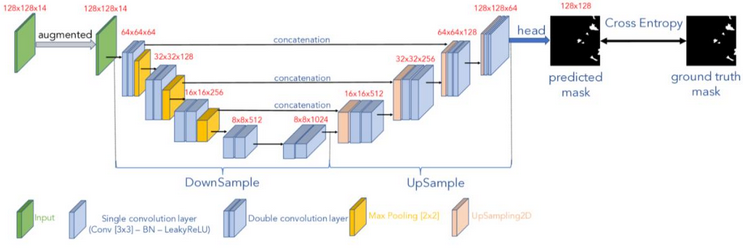
\includegraphics[width=0.98\textwidth]{unet}
 
    \end{tabular}
    \\
    \\
    The U-Net baseline comprises three main blocks: \textbf{down sample, up sample}, and head. Both down sample and up sample blocks make use of the same double convolution layer. The double convolution layer comprises two single convolution layers, each of which contains one convolutional layer (Conv[3×3]), one \textbf{Batch Normalization layer (BN)} [23], and one Leaky Rectified Linear Unit layer (LeakyReLU) [24]), as shown in Fig. 1. While the down sample block scales down the input images of 128×128×14 to 8×8×1024 by using the Max Pooling layer (MP[2×2]), the up sample block scales up the output of down sample block to 128×128×64 by applying Up Sampling 2D. The head block, which uses one dropout layer, one convolutional layer \textbf{(Conv[1×1]) and applies a Softmax function, helps to transform the output of up sample block to the image of 128×128}, referred to as the predicted mask. The predicted mask is compared with the ground truth mask using Cross Entropy as loss function.
    
    
\begin{table}[h]
    \centering
\begin{center}
\begin{tabular}{|p{2.57cm}|l|p{2.2cm}|}
\hline
\multicolumn{1}{|c|}{\textbf{Block}} & \multicolumn{1}{c|}{\textbf{Sub-blocks and Layers}} & \multicolumn{1}{c|}{\textbf{Output}} \\
\hline
\textbf{} & Initial Input & 128×128×14 \\
\textbf{DownSample} & Double convolution layer - MP layer[2×2] & 64×64×64 \\
 & Double convolution layer - MP layer[2×2] & 32×32×128 \\
 & Double convolution layer - MP layer[2×2] & 16×16×256 \\
 & Double convolution layer - MP layer[2×2] & 8×8×512 \\
 & Double convolution layer - Single convolution layer & 8×8×1024 \\
\hline
\textbf{UpSample} & Upsampling2D layer - Double convolution layer & 16×16×512 \\
 & Upsampling2D layer - Double convolution layer & 32×32×256 \\
 & Upsampling2D layer - Double convolution layer & 64×64×128 \\
 & Upsampling2D layer - Double convolution layer & 128×128×64 \\
\hline
\textbf{Head} & Dropout layer(0.2) - Conv layer[1×1] - Softmax & 128×128 \\
\hline
\end{tabular}
\end{center}
    \caption{The U-Net baseline architecture \cite{ra_unet}}
    \label{tab:abbreviations}
\end{table} 


		

		{\vfill \chapter*{\centering \vfill Chapter 3 \vfill}\vfill}
		\thispagestyle{empty}
		\newpage
		\label{Model Tarining}
		\section{Model Tarining }

		\label{Workflow Diagram}
		\subsection{Workflow Diagram}

\vspace{1cm}
\begin{center}

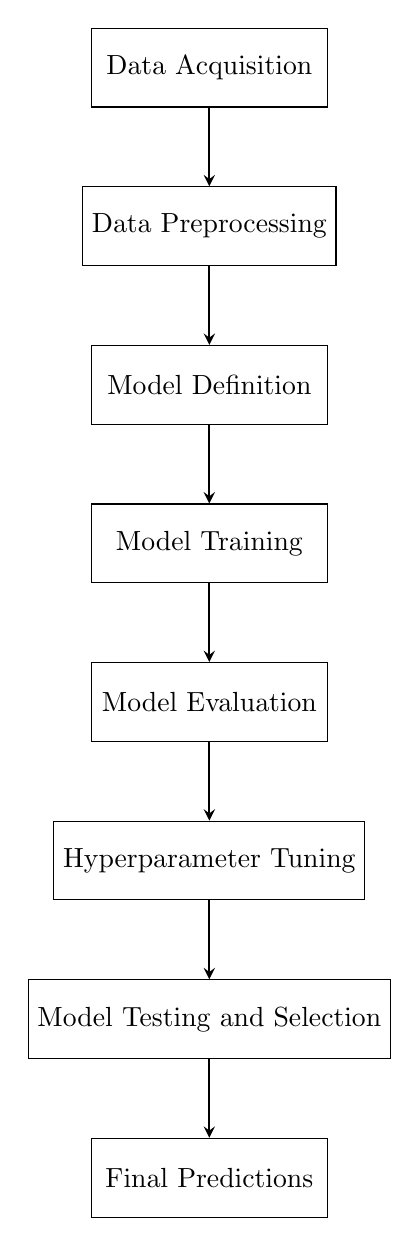
\begin{tikzpicture}[
    node distance=1cm,
    box/.style={draw, minimum width=3cm, minimum height=1cm, text centered},
    arrow/.style={thick,->,>=stealth}
]

\node (start) [box] {Data Acquisition };
\node (init) [box, below=of start] {Data Preprocessing };
\node (threads) [box, below=of init] {Model Definition };
\node (training) [box, below=of threads] {Model Training };
\node (capture) [box, below=of training] {Model Evaluation };
\node (process) [box, below=of capture] {Hyperparameter Tuning };
\node (update) [box, below=of process] {Model Testing and Selection};
\node (display) [box, below=of update] {Final Predictions };

\draw [arrow] (start) -- (init);
\draw [arrow] (init) -- (threads);
\draw [arrow] (threads) -- (training);
\draw [arrow] (training) -- (capture);
\draw [arrow] (capture) -- (process);
\draw [arrow] (process) -- (update);
\draw [arrow] (update) -- (display);

\end{tikzpicture}


\end{center}

\vspace{1cm}

		\label{Data Acquisition and Data Processing}
		\subsection{Data Acquisition and Data Processing}	We have collected almost four thousand satellite images in HDF5 format, each with dimensions of 128x128 and 14 channels. These channels include components such as RGB, slope, elevation, and near-infra-red (NIR). Out of these channels, we are utilizing six specific ones for our model: red (channel 3), green (channel 2), blue (channel 1), NIR (calculated using NIR - red) / (NIR + red)), slope (channel 12), and elevation (channel 13).

Before being used for model training, we normalize these six features to ensure their values fall within the range of -1 to +1. During training, we will use these features along with landslide images as labels.Our train-test split ratio is 4:1, where 20\% of the data will be reserved for validation purposes.\cite{gsch} 
	\\ \\

    		\label{Model Definition}
		\subsection{Model Definition}Here we have used U-Net architecture \cite{ra_unet} to define our model.The U-Net architecture  is specifically designed for biomedical image segmentation tasks due to its effectiveness in capturing fine-grained details while preserving spatial information. It comprises two main components: the contraction path and the expansive path.
		\subsubsection{Input Layer: } The model begins with an input layer that receives the satellite images for processing.
		\subsubsection{Contraction Path:}  Input images undergo a series of convolutional layers followed by max-pooling layers. This process extracts features and reduces spatial dimensions, facilitating the learning of hierarchical representations. Dropout layers are strategically inserted to mitigate overfitting.
		\subsubsection{Expansive Path:} Features obtained from the contraction path are up sampled using transpose convolutional layers. Concatenation layers merge these upsampled features with corresponding features from the contraction path, ensuring the preservation of spatial information. Additional convolutional layers refine the segmentation results, enhancing the model's ability to capture intricate patterns.
		\subsubsection{Output Layer:} The final layer employs a convolutional operation with a sigmoid activation function. This layer generates the output segmentation map, where each pixel represents the probability of belonging to the target class (e.g., landslide or non-landslide).
	\\ \\

    		\label{Model Training and Evaluation}
		\subsection{Model Training and Evaluation}We have trained multiple models using varying numbers of epochs and batch sizes to optimize efficiency while addressing common issues such as overfitting and underfitting. For model evaluation, we used metrics including N-Net model loss, precision, recall, and F1 score. \cite{jys} \cite{f1}
	\\ \\
	
	\begin{align*}
    \text{Precision} &= \frac{\text{True Positives}}{\text{True Positives} + \text{False Positives}} \\ \\
    \text{Recall} &= \frac{\text{True Positives}}{\text{True Positives} + \text{False Negatives}} \\ \\
    \text{F1 Score} &= 2 \times \frac{\text{Precision} \times \text{Recall}}{\text{Precision} + \text{Recall}} \\
\end{align*}

\subsubsection{Model Trained with 4 Epoch (Taking a small Amount of Data) }
		    \begin{tabular}{c c}
 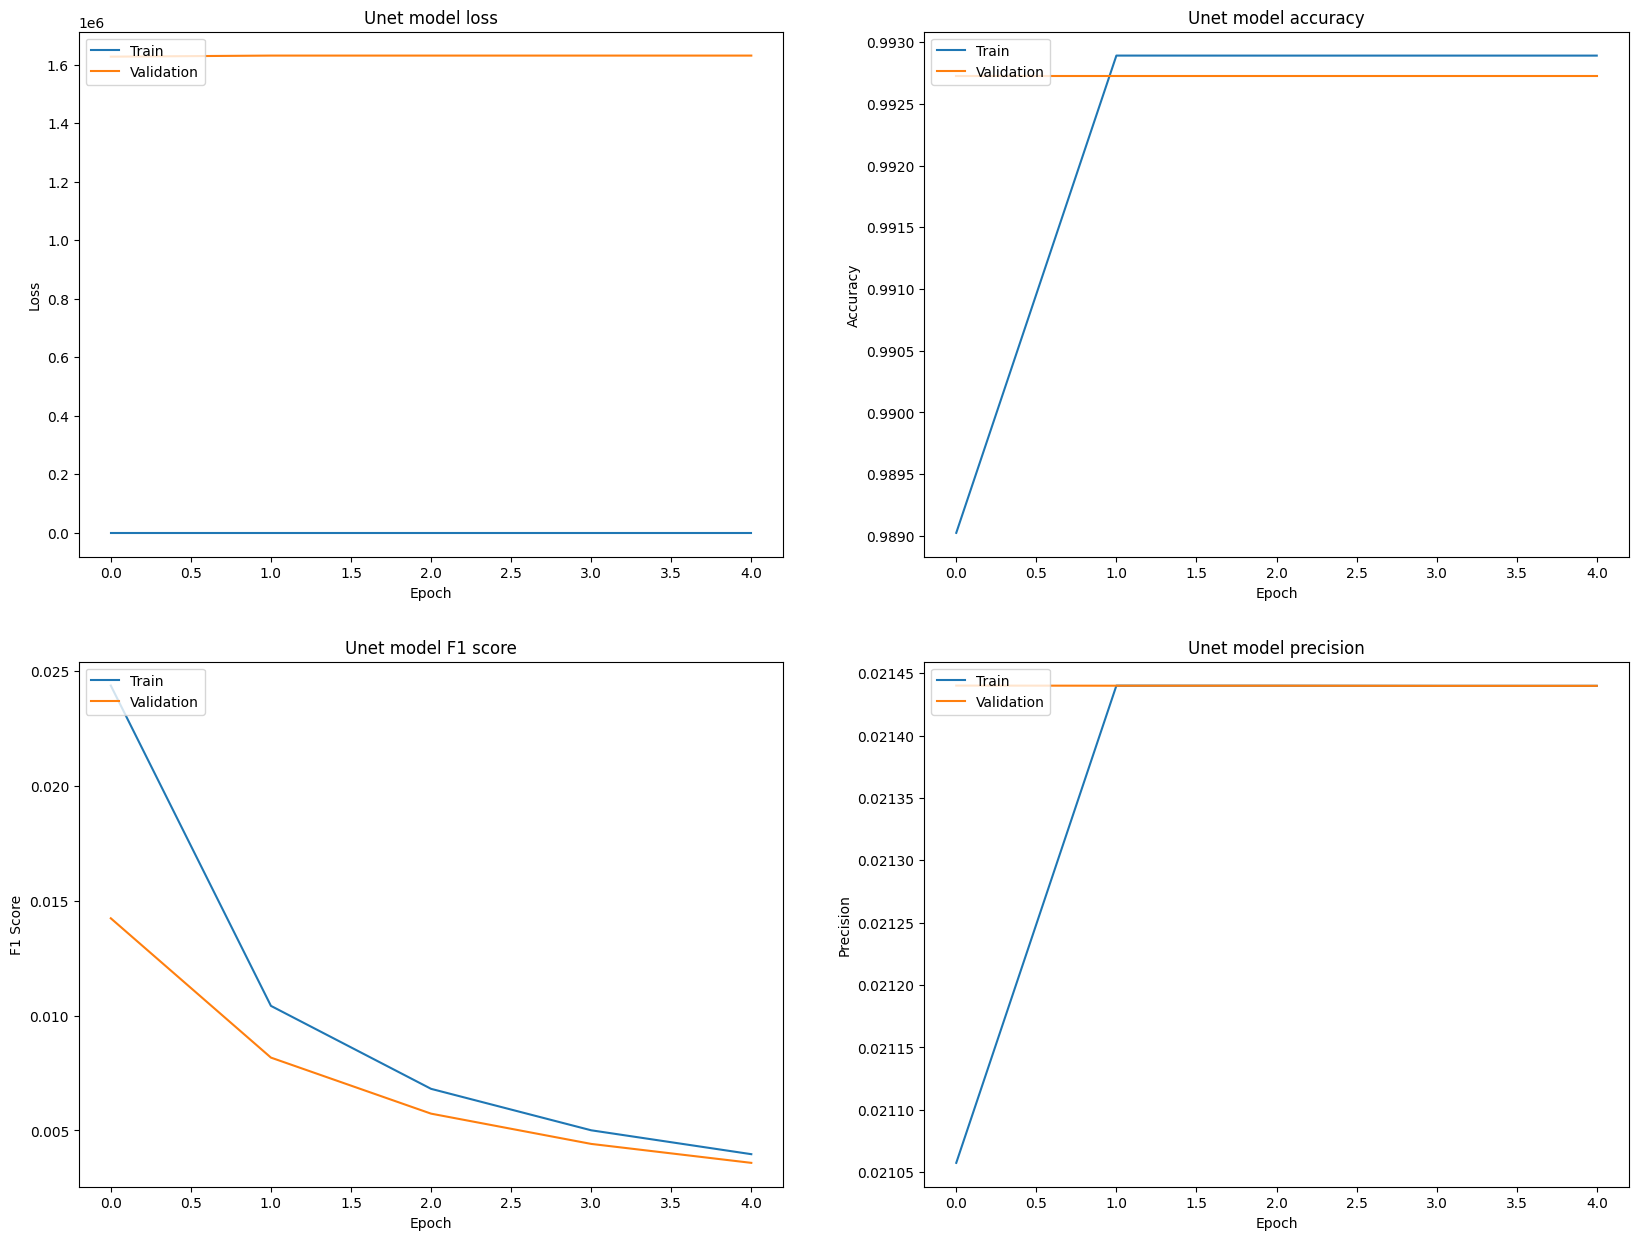
\includegraphics[width=0.97\textwidth]{4epoch}
    \end{tabular}
    \\
Here the difference between loss is very high so it is highly underfitted .


\subsubsection{Model with 10 Epoch and Batch size of 32  }
		    \begin{tabular}{c c}
 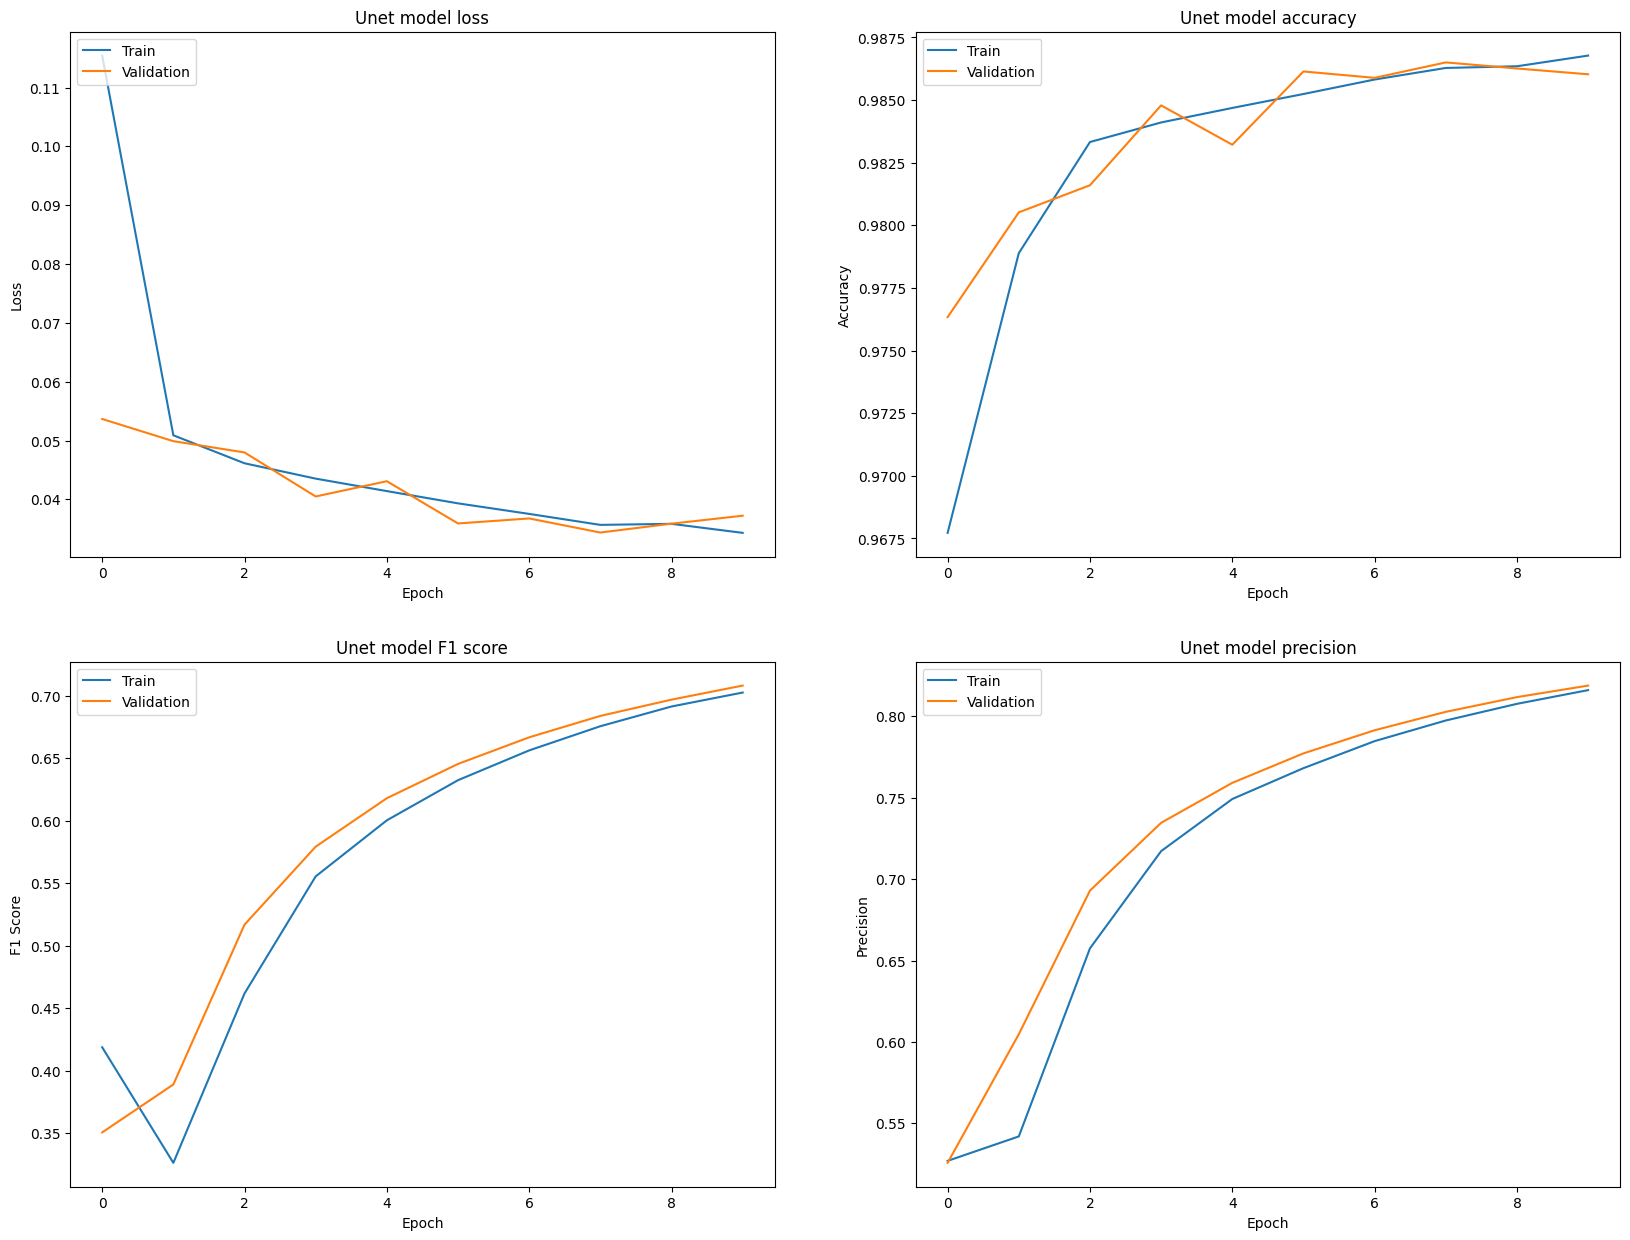
\includegraphics[width=0.97\textwidth]{10epoch}
    \end{tabular}
    \\
Here the difference between loss is less than before but significant so it is also underfitted we can see that with increasing the epoch the loss is reducing also the f1 score is increasing but not converged yet,so we need to increase our epoch numbers.

\subsubsection{Model with 100 Epoch and Batch size of 16  }
		    \begin{tabular}{c c}
 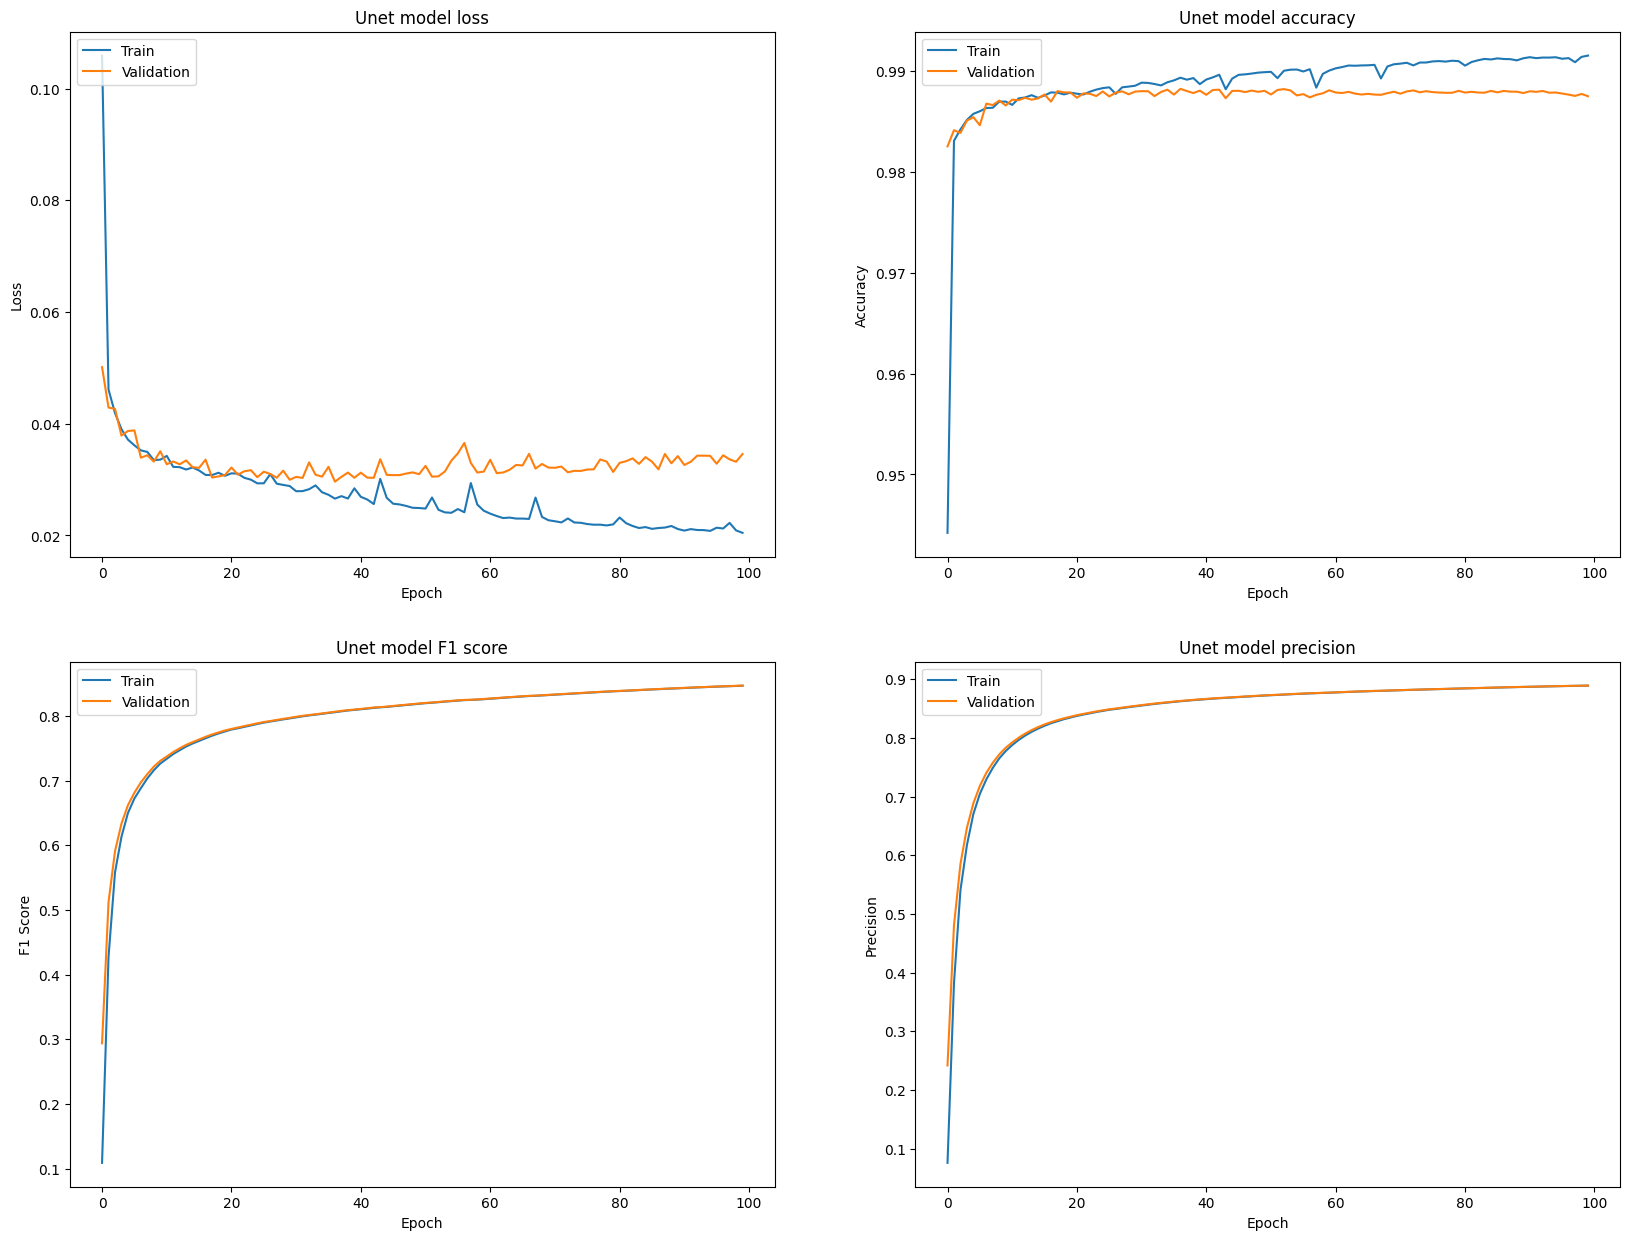
\includegraphics[width=0.97\textwidth]{100epoch}
    \end{tabular}
    \\
Here the difference between loss is much lesser also the model is neither underfitted nor overfitted so it is quite acceptable. We can see that with increasing the epoch the loss is reducing also the f1 score is increasing .Also the f1 score is converging around 80-90 epoch.

    		\label{Hyperparameter Tuning}
		\subsection{Hyperparameter Tuning}Hyperparameter tuning \cite{hyper}  refers to the process of adjusting the hyper parameters of a machine learning model to optimize its performance. Hyper parameters are configuration settings that are external to the model and cannot be learned from the data. Examples of hyper parameters include learning rate, batch size, number of layers in a neural network, and regularization parameters.
		
	In our hyper parameter tuning process, we increased the number of epochs to 160 while using a batch size of 32. To further optimize performance, we introduced a scheduler that reduces the learning rate by 5\% in each epoch after the 80th epoch. Additionally, we implemented early stopping based on the F1 score, with a minimum delta of 0.1\% and a patience of 20 epochs. This means that if the model's F1 score does not increase by at least 0.1\%, training will continue for an additional 20 epochs. If no improvement is observed within this timeframe, training will be halted and model with best f1 score during these time will be saved.	
		 \\
		 \begin{tabular}{c c}
 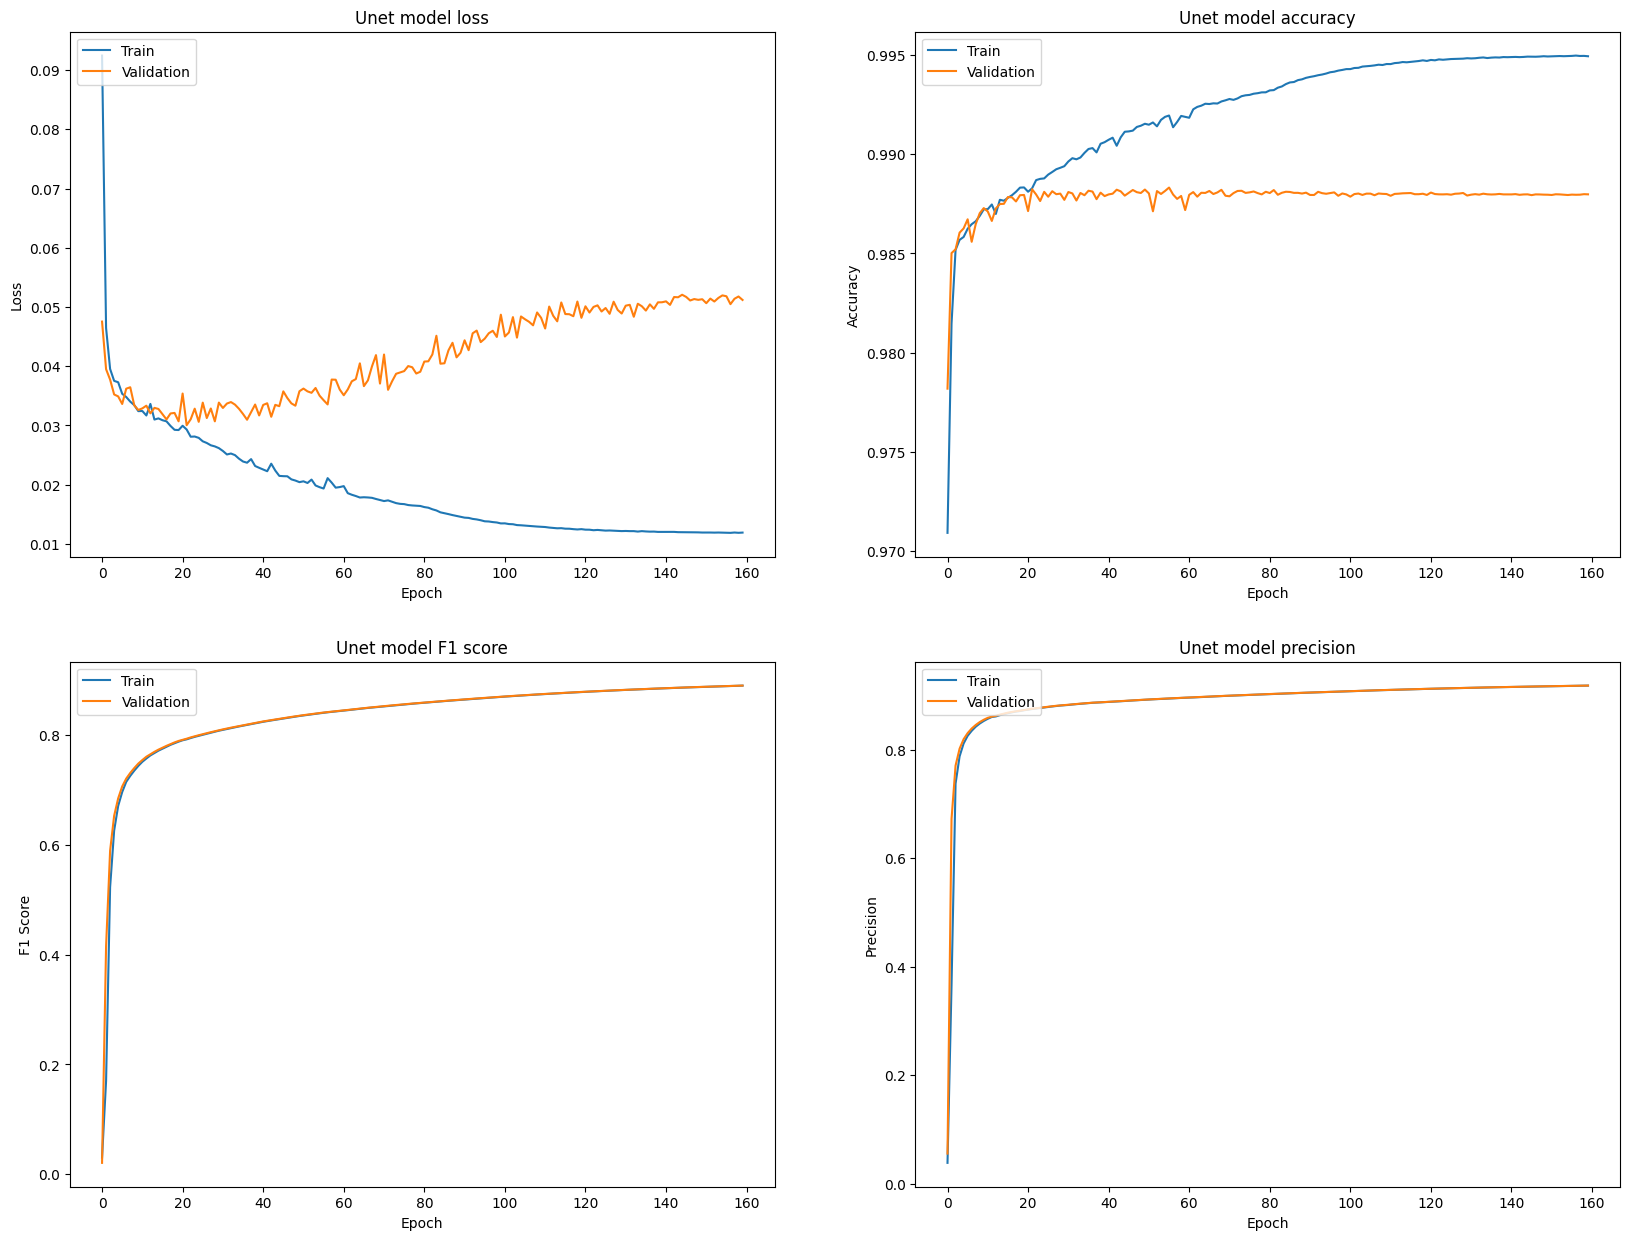
\includegraphics[width=0.97\textwidth]{160epoch}
    \end{tabular}
    \\
    Here we can see the accuracy is almost 90\% but if we carefully look train and validation loss we will observe the train loss is decreasing while validation loss is increasing .So the model is now giving much more better perdition on train data but bad results on validation data. Hence it is overfitted .Therefore, our previous model trained with 100 epochs performs better compared to this one. \\
		 

		\label{Model Testing and Selection}
		\subsection{Model Testing and Selection} In model testing and selection we will use f1 score \cite{f1}  ,precision, U-Net loss from previous discussion including confusion matrix to evaluate our classification model.
		A confusion matrix is a table used in classification to evaluate the performance of a machine learning model. It allows visualization of the performance of an algorithm by presenting the number of correct and incorrect predictions made by the model compared to the actual outcomes. 
		In a confusion matrix, the rows represent the actual classes, while the columns represent the predicted classes. It is typically organized as follows:
		\begin{itemize}
		\item \textbf{True Positive (TP):} Predicted positive and actually positive.
    \item \textbf{False Positive (FP):} Predicted positive but actually negative (Type I error).
    \item \textbf{True Negative (TN):} Predicted negative and actually negative.
    \item \textbf{False Negative (FN):} Predicted negative but actually positive (Type II error).
		\end{itemize}
		Now considering these properties we will evaluate our models :\\
		

		    \begin{tabular}{c c c}
 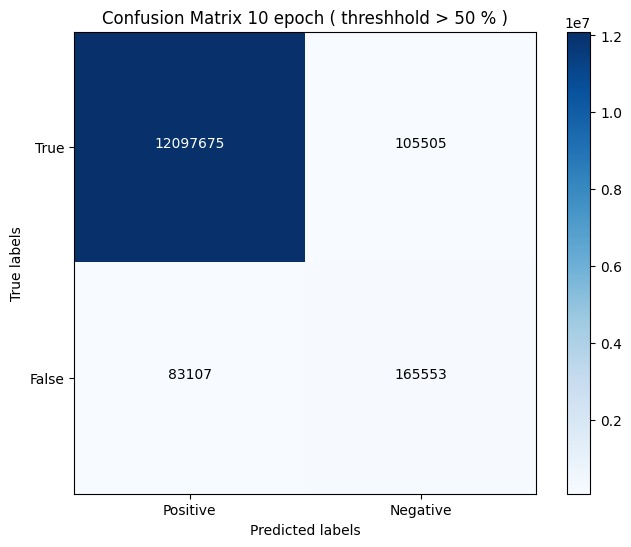
\includegraphics[width=0.31\textwidth]{10cf}&
 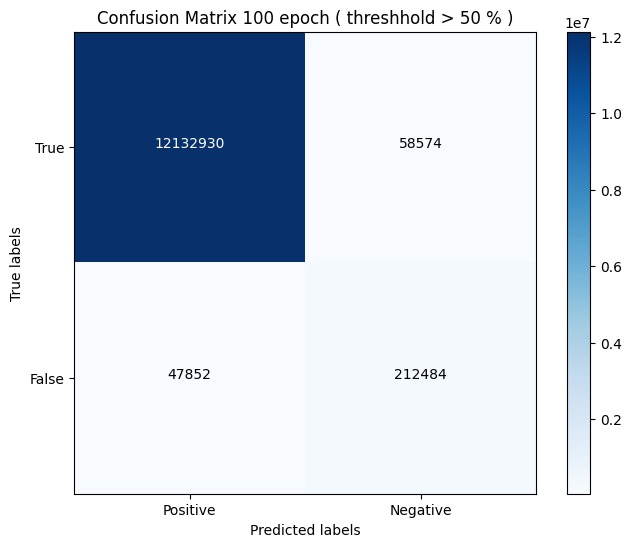
\includegraphics[width=0.31\textwidth]{100cf}&
 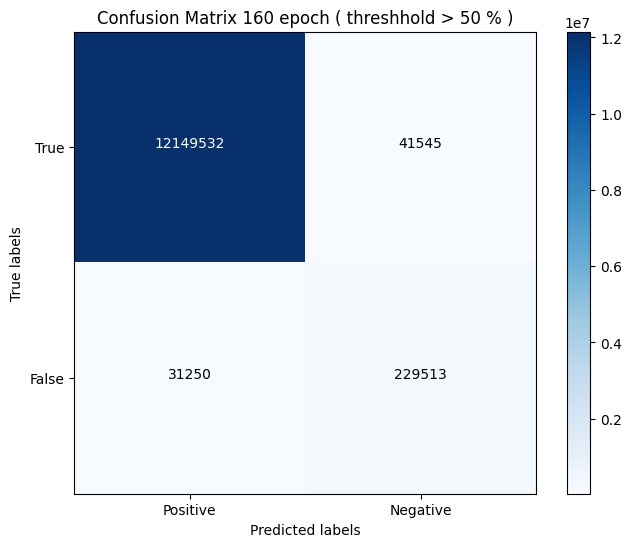
\includegraphics[width=0.31\textwidth]{160cf}
    \end{tabular}
    In these testing 160 epoch's model giving us most true positive results and 10 epoch's is giving least while 100 epoch is quite near to 160 epoch's true positive perdition.In this way if we consider other parameters then 160 epoch's model is slightly better than of 100 epoch's model but there was overfitting related issue in 160 epoch's model .So considering all these points model trained with 100 epoch with batch size of 16 is selected.\\   
    
    
    \subsubsection{Threshold Selection for Classification}
    
In classification tasks, selecting the threshold is pivotal for model performance and interpreting results. It defines the boundary between positive and negative predictions, affecting metrics like accuracy, precision, recall, and F1 score. Lower thresholds raise sensitivity but may reduce specificity, and vice versa for higher thresholds.
 Ultimately, threshold selection requires careful consideration and experimentation to optimize performance and meet application objectives. This can be effectively illustrated using a confusion matrix, which summarizes the model's predictions against ground truth labels.
 
\begin{itemize}
		\item \textbf{Prediction for Balanced (50\%) Threshold Values}
\end{itemize}  
		\begin{tabular}{c}
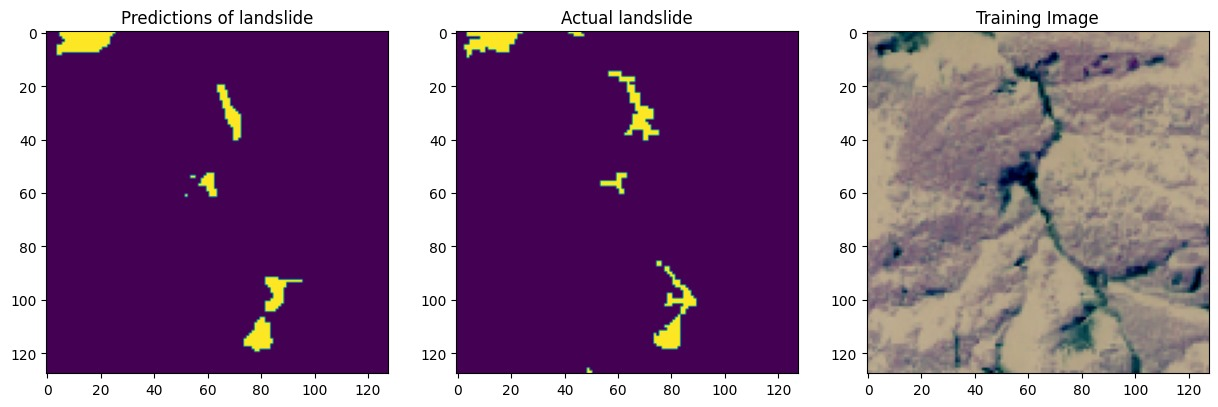
\includegraphics[width=0.99\textwidth]{th_balanced}
    \end{tabular}    
\begin{itemize}
		\item \textbf{Prediction for Lower Threshold Values}
\end{itemize}  
		\begin{tabular}{c}
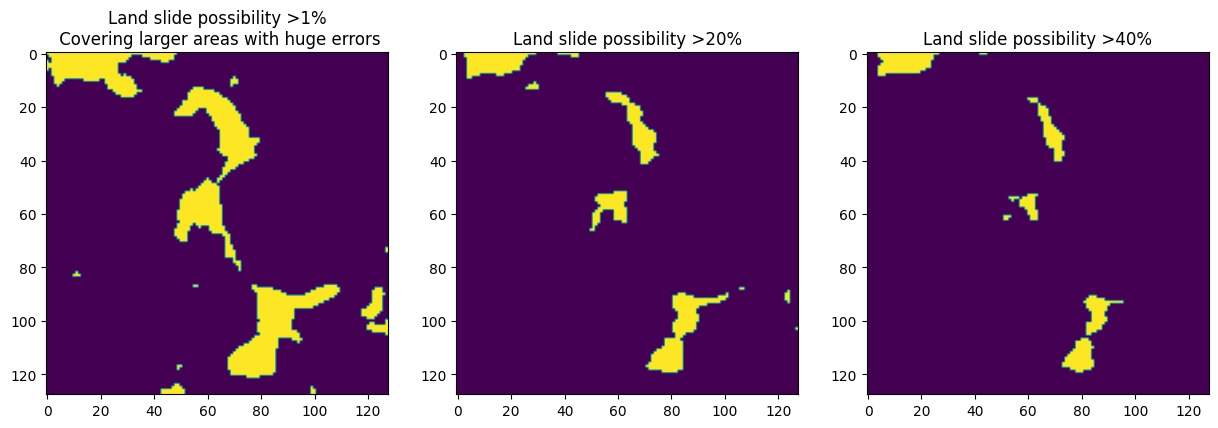
\includegraphics[width=0.99\textwidth]{th_lower}
    \end{tabular}
   \begin{itemize}
		\item \textbf{Prediction for Higher Threshold Values}
\end{itemize}  
		\begin{tabular}{c}
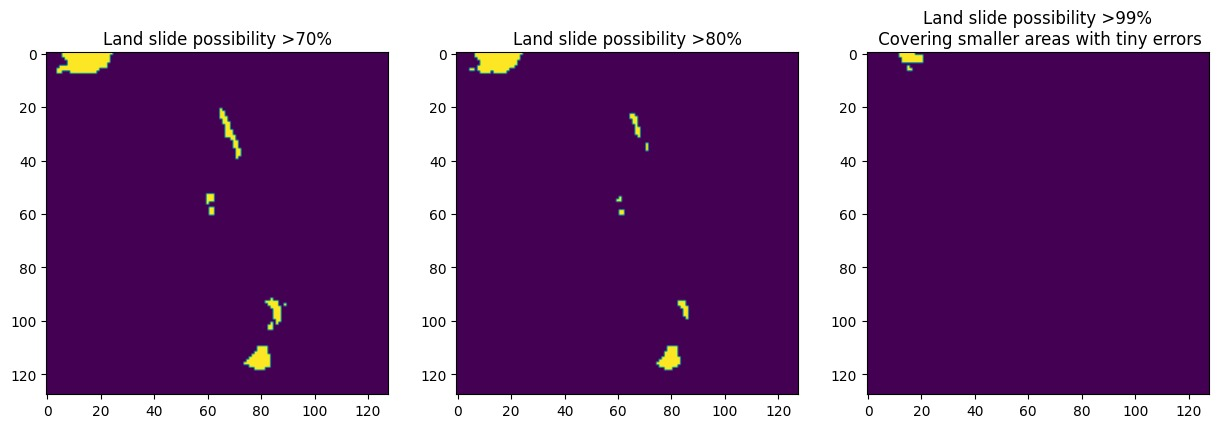
\includegraphics[width=0.99\textwidth]{th_higher}
    \end{tabular}
    
\begin{itemize}
		\item \textbf{Confusion Matrix for 1 \%, 99 \%  and 50 \% Threshold}
\end{itemize}  
		    \begin{tabular}{c c c}
 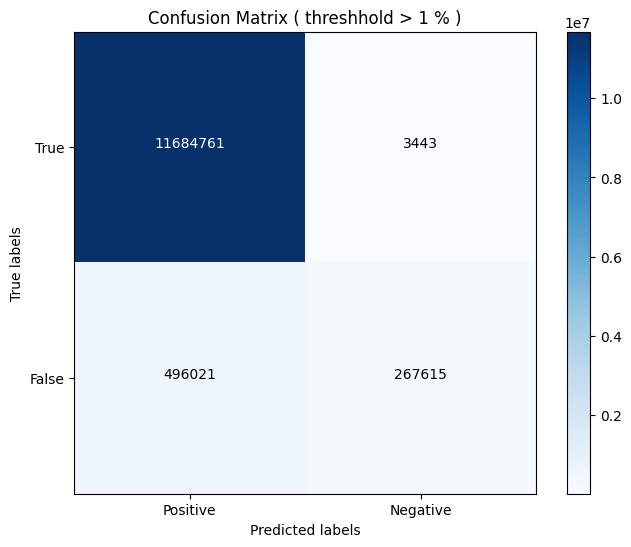
\includegraphics[width=0.31\textwidth]{th1}&
 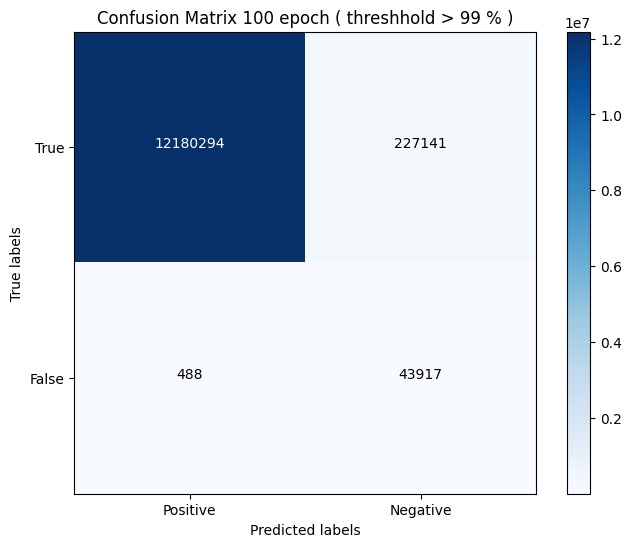
\includegraphics[width=0.31\textwidth]{th99}&
 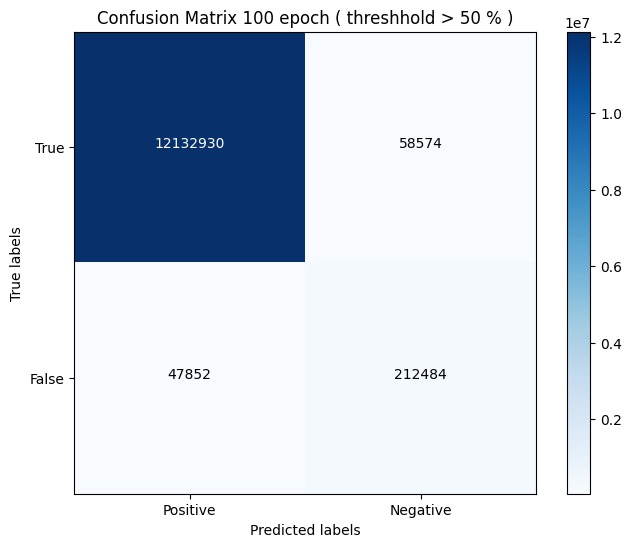
\includegraphics[width=0.31\textwidth]{th50}
    \end{tabular}
So here we can see that in first one our total positive prediction is highest and it is lowest in the second one while balanced in the third confusion matrix.So with lower threshold our model is labelling much more areas for landslide and while increasing the threshold landslide area is decreasing but the accuracy is increased.As where first confusion matrix giving us huge amount of false positive perdition and second one is giving least as the threshold or cut off is 99\% where third matrix it again balanced .

Also if we compare prediction with 50\% threshold value with actual landslide then we can see that around 50\% threshold value we are getting more accurate prediction so threshold is selected as 50\%  for classification of landslide region or not .



				{\vfill \chapter*{\centering \vfill Chapter 4 \vfill}\vfill}
				\thispagestyle{empty}
	\newpage
	\label{Performance Analysis}
	\section{Performance Analysis}{
		We utilized a feature set comprising six key variables: red (R), green (G), blue (B), slope, elevation, and normalized difference vegetation index (NDVI) to predict landslide occurrences. These features were carefully selected based on their relevance to terrain characteristics and their potential impact on landslide susceptibility.

Additionally, to assess the model's performance and generalization capability, we conducted evaluations on a separate validation dataset. This dataset was distinct from the one used for model training, ensuring an unbiased assessment of the model's predictive accuracy and robustness across unseen data samples. By validating the model on an independent dataset, we aim to provide more reliable insights into its real-world performance and its ability to generalize to new environmental conditions.

 	\begin{itemize}
    \item \textbf{4 Epoch with batch size of 16 and 25\% data only} , 
    \item \textbf{10 Epoch with batch size of 32} and all data used, 
    \item \textbf{38 Epoch with batch size of 32 and hypertuned},
    \item \textbf{85 Epoch with batch size of 16 and hypertuned },
    \item \textbf{100 Epoch with batch size of 16},
    \item \textbf{160 Epoch with batch size of 32 and hypertuned using reducing learning rate of 5\% after 80 epoch}
\end{itemize}
	\label{Test Results of Functionalities}
	\subsection{Test Results of Functionalities}
	\begin{table}[h]
    \centering
    \begin{tabular}{|c|c|c|c|}
        \hline
        \textbf{Epoch } & \textbf{Batch Size} & \textbf{Hypertuned} & \textbf{F1 Score} \\
        \hline
        4 & 16 & No & 0.5\% \\
        \hline
        10 & 32 & No & 80\% \\
        \hline
        38 & 32 & Yes & 81\% \\
        \hline
        85 & 32 & Yes & 84\% \\
        \hline
        100 & 16 & No & 85\% \\
        \hline
        160 & 32 & Yes & 89\% \\
        \hline
    \end{tabular}
    \caption{Test Results of Different Model}
    \label{tab:Test Results of Different Model}
\end{table}
From the Table we can see that the f1 score of model with hypertuned is heighest .	
	}	
\newpage

\thispagestyle{empty}
 \newpage
			{\vfill \chapter*{\centering \vfill Chapter 5 \vfill}\vfill}
		\thispagestyle{empty}
	
	\newpage
	\label{Conclusion and Future Scope}
	\section{Conclusion and Future Scope}

	\subsection{Conclusion}	The deployment of the UNet architecture for landslide detection using satellite imagery and deep learning represents a significant advancement in geospatial technology. This method holds immense potential not only for the scientific community but also for the broader society. By enabling more accurate and timely predictions of landslides, it can play a crucial role in safeguarding lives and property. The ability to quickly analyse vast areas and identify vulnerable regions allows for efficient allocation of resources and better preparation for potential disasters.

Furthermore, this approach can assist in the development of more resilient infrastructure and inform urban planning, ensuring that communities are built with consideration for natural hazards. It also contributes to precision agriculture by helping monitor land conditions, thus supporting sustainable farming practices. In the face of climate change, the insights provided by this technology are invaluable for adaptation strategies, helping societies to anticipate and mitigate the impacts of extreme weather events.

Overall, the integration of UNet architecture in landslide detection is a testament to how cutting-edge technology can be harnessed for the greater good, offering a proactive solution to one of the many challenges posed by our changing environment. It exemplifies the transformative power of artificial intelligence in enhancing our ability to protect and nurture the planet and its inhabitants.	
	
	
	
	\subsection{Future Scope}	The \mytitle , presents promising avenues for future research and development: 

		\begin{itemize}
		
    \item Improved Accuracy and Efficiency: With ongoing advancements in machine learning algorithms and satellite imaging technology, the accuracy and efficiency of landslide detection models are expected to improve further. Future research can focus on refining existing models, exploring novel architectures, and leveraging larger and more diverse datasets to achieve even better performance.

    
    \item Integration with Disaster Management Systems: Landslide detection systems can be integrated with disaster management systems at local, regional, and national levels. These systems can provide early warnings and real-time monitoring of landslide-prone areas, allowing authorities to take timely preventive measures and mitigate potential damage to lives and infrastructure.
 
    
    \item Precision Agriculture and Environmental Monitoring: The techniques developed for landslide detection can be adapted and applied to other domains such as precision agriculture and environmental monitoring. By analysing satellite imagery, machine learning models can identify areas prone to soil erosion, water logging, or other environmental hazards, enabling farmers and environmental agencies to implement targeted interventions and sustainable land management practices.
 
    \item Urban Planning and Infrastructure Development: In urban areas, landslide detection models can inform urban planners and policy-makers about the suitability of land for infrastructure development, construction projects, and urban expansion. By identifying areas at risk of landslides, these models can help prevent disasters, reduce economic losses, and ensure the safety of residents.
 
    \item Climate Change Adaptation: Climate change is expected to influence the frequency and intensity of natural disasters, including landslides. As the climate continues to change, there will be an increasing need for reliable tools and methods for landslide detection and risk assessment. Machine learning-based landslide detection models can play a crucial role in adapting to these changes and developing resilient infrastructure and land-use policies.

    \item Global Scale Monitoring: Satellite imagery provides a unique opportunity to monitor landslide activity on a global scale. By analysing satellite data collected over extended periods, researchers can gain insights into long-term trends, regional variations, and the impact of environmental factors on landslide occurrence. This global perspective can inform policy decisions, guide resource allocation, and support international efforts to address landslide risk.
\item Crowd-sourced Data and Citizen Science: With the proliferation of mobile devices and crowdsourced data collection platforms, there is potential to engage citizens in landslide monitoring and data collection efforts. Citizen science initiatives can complement traditional satellite-based monitoring systems by providing ground-level observations, real-time reports, and community-based solutions to landslide risk management. 
	
	\end{itemize}

	

	\newpage



\bibliographystyle{plain} 
\bibliography{references} 

	
\end{document}